\section{Numerical study}\label{sec:results}
We use $\delta=0.05$, $\kappa=0.95$ and the finite allocation grid
$b/E\in\{0.4,0.6,0.8\}$. Eight cases use
$a\in\{0.3,0.6\}$, $u\in\{0.125,0.2\}$, $E=0.025$,
$c_\psi\in\{1,32\}$ and $N=20$. Two further cases use
$a=0.6$, $u\in\{0.25,0.4\}$, $E=0.05$, $c_\psi=1$ and $N=12$.
The full serial-query caps are $c_\psi+4N+1$ for each problem.
All cases satisfy $u>4E$, excluding the prior-midpoint solution.
The parameter $c_\psi$ is a sensitivity parameter of the cost model;
we do not claim that preparing the simple matrix-audit input costs 32
queries on actual hardware.

\paragraph{Candidates and certificates.}
The comparison families are endpoint-nulling power $(1-x)^n$,
quartic-power $(1-x^2)^t$, endpoint-nulled cosine-Taylor products
$(1-x)(1-0.72x^2)^t$, and the classical low-pass Chebyshev polynomial
\[
 (1-x)\frac{T_{n-1}((2x-1-v)/(1-v))}
                  {T_{n-1}(-(1+v)/(1-v))},
 \quad v\in\{.04,.08,.16,.28,.42,.60,.78\}.
\]
The degree is always measured in $x=\lambda$ and then converted to signal
queries identically. Normalization, target positivity and bias are
certified for every reported candidate. Optimized candidates use initial
17-target/65-tail/129-support grids, with up to three exchange rounds
against denser grids. The LP design bias is $0.98b$; the continuous
polynomial certificate uses $0.99b$, leaving $0.01b$ for realization error.
The verifier can reject a gridded optimum, so the selected design is the
best continuously certified candidate among those attempted; its
optimality gap remains controlled by the independent dual lower bound.

\begin{table}[tb]
\centering\small
\begin{tabular}{rrrrrlrrr}
\toprule
$a$ & $u$ & $E$ & $c_\psi$ & $n$ & Response & $b$ & $J^{\rm up}$ & Gap \\
\midrule
0.30 & 0.125 & 0.025 & 1 & 8 & LP & 0.015 & 1.79e+08 & 9.5\% \\
0.30 & 0.125 & 0.025 & 32 & 8 & LP & 0.015 & 3.47e+08 & 9.5\% \\
0.30 & 0.200 & 0.025 & 1 & 8 & LP & 0.020 & 1.71e+09 & 23.9\% \\
0.30 & 0.200 & 0.025 & 32 & 8 & LP & 0.020 & 3.31e+09 & 16.2\% \\
0.60 & 0.125 & 0.025 & 1 & 4 & LP & 0.015 & 3.27e+06 & 21.4\% \\
0.60 & 0.125 & 0.025 & 32 & 4 & LP & 0.015 & 9.19e+06 & 3.7\% \\
0.60 & 0.200 & 0.025 & 1 & 4 & LP & 0.015 & 1.02e+07 & 7.5\% \\
0.60 & 0.200 & 0.025 & 32 & 5 & LP & 0.015 & 2.72e+07 & 5.6\% \\
0.60 & 0.250 & 0.050 & 1 & 2 & Cheb. & 0.030 & 5.1e+05 & 4.9\% \\
0.60 & 0.400 & 0.050 & 1 & 3 & LP & 0.030 & 1.98e+06 & 7.4\% \\
\bottomrule
\end{tabular}

\caption{Prior-only selections. $n$ is Gram-polynomial degree. ``LP'' is a
certified optimized polynomial; ``Cheb.'' is a certified member of the
tested Chebyshev grid. The gap is $100(J^{\rm up}/\min J^{\rm lo}-1)$,
relative to the endpoint-nulling class, degree cap and finite allocation
grid, not to all quantum estimators.}
\label{tab:selection}
\end{table}

The selections have certified cost factors between $1.0372$ and $1.2394$
relative to the restricted optimum lower bound. Most selected responses
come from the coupled LP, but the $a=0.6,u=0.25,E=0.05$ case selects the
tested Chebyshev response instead. Thus the implementation does not
automatically prefer the newly optimized family. Power and Chebyshev
candidates are certified in all ten cases. No quartic-power or
cosine-Taylor candidate passed the requirements within the searched
degree/parameter grid in these harder cases; this is recorded as absence
of a certified candidate, not a proof of impossibility for all tunings.
Relative to the selected upper costs, the tested power upper costs range
from approximately $1.44$ to $4.36$ times as large. These are comparisons
of guaranteed costs in the common model, not empirical runtime speedups.

\begin{figure}[tb]
\centering
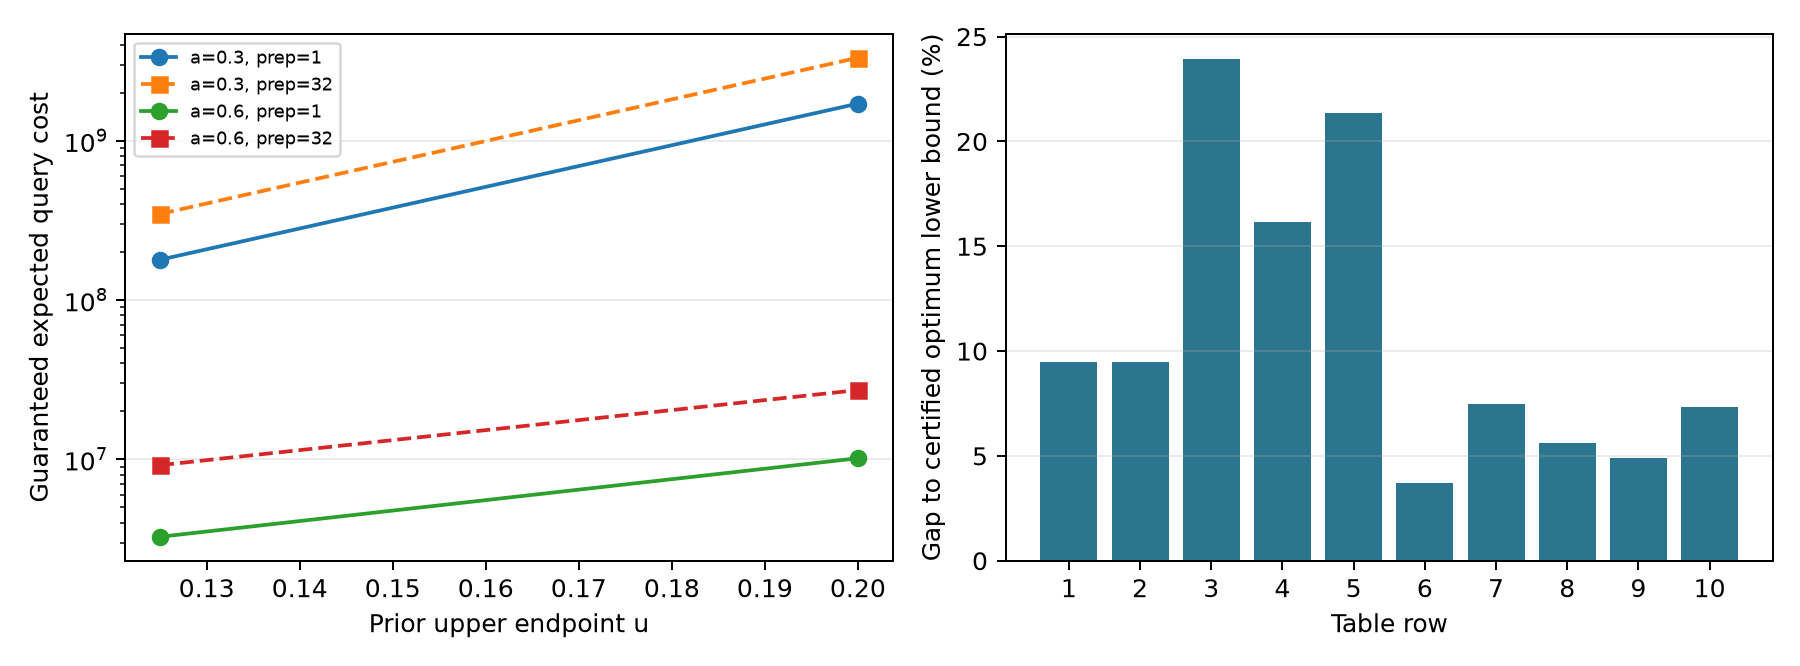
\includegraphics[width=\linewidth]{../../figures/selection_costs.png}
\caption{Guaranteed expected query costs and a posteriori gaps for the
main cases. Different preparation costs are separate specified problems;
all candidates within each problem share its cap and oracle accounting.}
\label{fig:costs}
\end{figure}

\paragraph{A preparation-cost-dependent switch.}
For $a=0.6,u=0.2,E=0.025$ and $b=0.015$, preparation cost one selects
degree four, whereas preparation cost 32 selects degree five. Both use
the same accepted-copy sample count. The latter response has greater
guaranteed acceptance, enough to compensate for the additional queries
when input preparation is expensive. For the ideal polynomial responses,
exact transmission intervals give
the crossover interval reported in the supplementary numerical summary;
the central displayed guaranteed-cost crossover is approximately $12.34$
preparation-query units. This comparison concerns two fixed certified
polynomials; it is not a claim that these are the only optimal candidates
at every intermediate preparation cost.

\begin{figure}[tb]
\centering
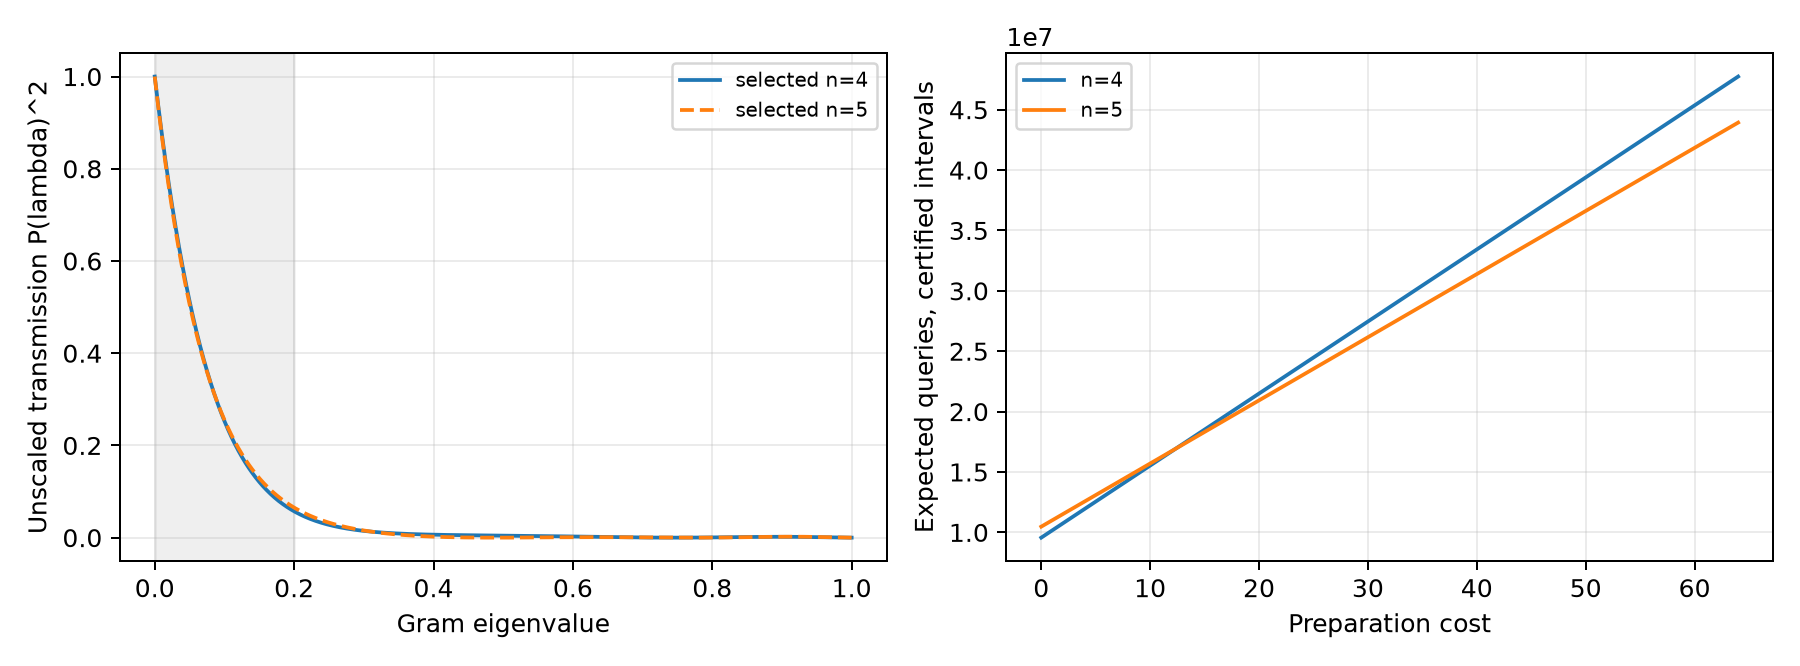
\includegraphics[width=\linewidth]{../../figures/selection_crossover.png}
\caption{Two selected responses for the same prior and bias allocation.
The shaded spectral interval is the supplied prior. Their certified
cost lines exchange order as preparation cost increases; transmission
enclosures produce the narrow bands.}
\label{fig:crossover}
\end{figure}

\paragraph{The price of prior width.}
Figure~\ref{fig:prior} compares the certified target transmissions with
the unrestricted bound of Proposition~\ref{prop:prior}. None exceeds
the function-level limit. For example, at $a=0.3$ widening the prior
from $0.125$ to $0.2$ at $E=0.025,c_\psi=1$ increases the selected
guaranteed cost from about $1.79\times10^8$ to $1.71\times10^9$ queries.
These large absolute costs do not demonstrate practicality; they
illustrate the limitations of this robust filtered-mean protocol.

\begin{figure}[tb]
\centering
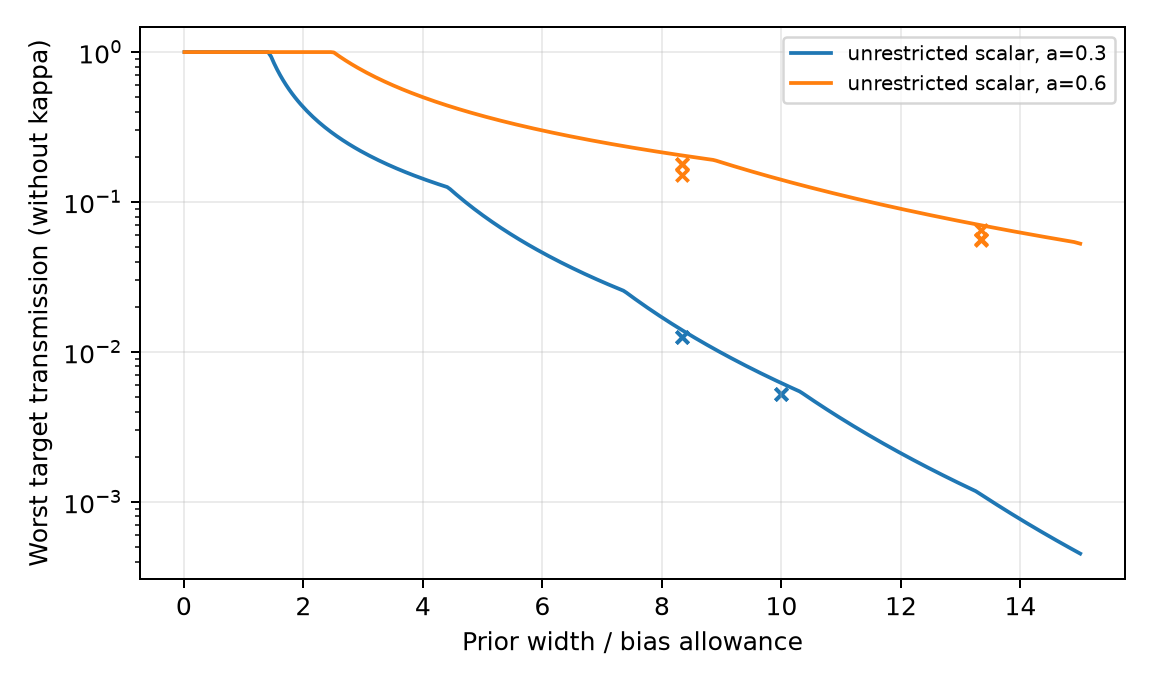
\includegraphics[width=.72\linewidth]{../../figures/selection_prior_limit.png}
\caption{The exact unrestricted target-transmission limit as a function
of prior width divided by bias allowance, and certified polynomial
transmissions (crosses). The margin $\kappa$ is excluded from both
quantities here.}
\label{fig:prior}
\end{figure}

\paragraph{Phase and matrix audits.}
All ten selected whole polynomials were synthesized successfully.
The largest certified continuous amplitude error of the saved phase
responses is $3.63\times10^{-16}$. Each satisfies the reserved mean-bias
allowance; the certified worst-success correction changes the cost
by less than a factor $1+1.4\times10^{-14}$.
These statements apply to the ideal signal convention, not to hardware
rotation synthesis or noisy block-encodings.

For each selection we also construct an eight-dimensional positive
matrix $B$ with a minimum in the supplied interval and use the fixed
computational input $\ket0$. A Householder rotation in the synthetic
generator controls its overlap promise; the estimator never receives
that rotation or the true eigenvalues for its design. One case of each
pair includes an excitation only $10^{-7}$ above the minimum.
We apply every QSP phase to the full $16\times16$ signal matrix and
explicitly form the $32\times32$ extraction unitary. The maximum
response-matrix error against the polynomial target is
$5.55\times10^{-16}$ and the maximum unitarity residual is
$6.33\times10^{-15}$. This is an exact-oracle matrix simulation, not
physical-gate compilation.

Across 1,000 held-out scalar spectral inputs (seed 20261027), the
guaranteed bias and success bounds held. A further 2,000 aggregate
Bernoulli/negative-binomial replicates for the full matrix examples
(seed 20261028) had no confidence failures at the requested error.
The confidence guarantee comes from the theorem; observing zero finite
sample failures is only a consistency check. All coefficients, phases,
input matrices, sample settings and exact certificates are included.
